
\section{The pseudogap vs. the coherent state}

The phase diagram for the cuprates, when hole doping is the tuning parameter, appears to be universal, however, at the time of writing, is somehwhat more complicated than that of a typical pnictide\footnote{In general there is more variation in the phase diagram amongst pnictide materials, however there are less features in these diagrams when compared to the cuprates}. With reference to the schematic cuprate phase diagram shown in figure~\ref{Fig:Intro:UniversalCupratePhaseDiagram} we see several temperature scales that may or may not be of interest to the underlying causes of \highTc superconductivity.
\begin{figure}[htbp]
    \begin{center}
        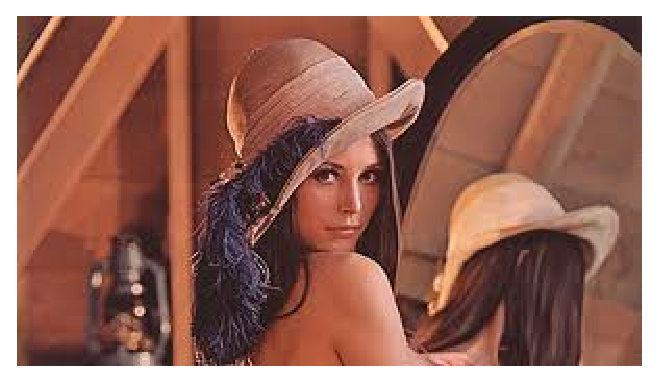
\includegraphics[scale=0.7]{Misc/TODO}
        \caption{A schematic phase diagram of a series of hole-doped cuprates}
        \label{Fig:Intro:UniversalCupratePhaseDiagram}
    \end{center}
\end{figure}
From the standpoint of conventional superconductivity, the first striking feature is the proximity of an antiferromagnetic phase to the superconducting region. Even without actual temperature labels, it becomes clear that if this was a phonon mediated superconductor, the pairing must be strong in order to overcome the strong spin-density wave scattering that results in the anitferromagnetic state.

Another interesting region, one that is not present in the pnictides, is that below the $T^*$ temperature scale on the underdoped side of the superconducting dome. In this region, an energy gap opens up in the excitation spectra but without any sign of the Meissner effect. This region is known as the \textit{pseudogap}. Some aspects of the pseudogap lead us to believe that it is closely related to the superconducting gap such as the fact that it shares the gap symmetry and is of a similar magnitude, and there have been proposals that the pseudogap is a precursor state to superconductivity \TODO{Read more}. However research involving the Bristol group has shown evidence that phase fluctuations rather than the pseudogap in particular are the neceesary precursors for the cuprate superconducting condition\cite{Rourke2011}.

\subsection{Anisotropic scattering}


